% \section{Additional Details and Experiments}
% %

% \subsection{\ourmethod{} can approximate the frequency response of digital filters}

% We experimentally verify whether \ourmethod{} can approximate the input--output map of digital filter admitting a state--space representation, with improved generalization over baseline models given test inputs of unseen frequencies.

% We generate a dataset of $1028$ sinusoidal signals of length $200$
% \[
% x(t) = \sin{(2\pi \omega t})
% \]
% where $\omega \in [2, 40]~\bigcup~[50, 100]$ in the training set and $\omega \in (40, 50)$ in the test set. The outputs are obtained by filtering $x$, i.e., $y = \mathcal{F}(x)$  where $\mathcal{F}$ is in the family of digital filters. 

% We introduce common various sequence-to-sequence layers or models as baselines: the original S4 diagonal plus low--rank \citep{gu2021efficiently}, a single layer LSTM, a single 1d convolution (Conv1d), a dense linear layer (NLinear), a single self--attention layer. All models are trained for $800$ epochs with batch size $256$, learning rate $10^{-3}$ and Adam. We repeat this experiment for digital filters of different orders \citep{oppenheim1999discrete}. The results are shown in Figure \ref{fig:dsp_synthetic}. \ourmethod{} learns to match the frequency response of the target filter, producing the correct output for inputs at test frequencies. 

% %
% \paragraph{State as memory}
% %
% In deep state space models, $x\in\R^n$ is the state of a system with a recurrence defined as some matrix $\zA$ (not necessarily in companion form). Given an initial state $x$, for how many recurrence steps can the system \textit{remember} it? We reason about $x$ as model memory to highlight its role as a latent vector of sufficient information to predict an output as $y = cx$.
% %

% If the recurrence is defined as a forward shift $\zS$, $\zS^n = \0$ and thus the model contains information about the initial condition only for for $n$ steps. This notion can be made formal by noting that if the recurrence is defined as contractive operator i.e. eigenvalue $|\lambda(\zA)_{\text{max}}| < 1$, \textbf{or} $\zA$ is nilpotent, after convergence to the fixed--point $x^* = \zA x^*$ (which exists by Banach's fixed--point theorem) there is no information left about the initial condition: all inputs eventually converge to the same fixed--point. If the recurrence is full--rank and not a contraction, the state will never reach a fixed--point and less can be said about the state as a latent vector of fading memory.
% %

% Keeping the recurrence at the edge of stability (maximum eigenvalue close to $1$) ensures a longer transient phase and thus a longer effective memory. 
% %

% \subsection{{\color{red!70}Initialization for Long--Range Memory}}
% %
% A crucial ingredient for the success of deep SSMs for long--range sequences is an initialization that promotes diversity in the temporal scales of the input signals attended to by different heads of the model. 

% For example, ${\tt S4D}$ 


% \[
% x^*: x^* = {\tt shift}(x) + px[-1]    
% \]

%




% In example, it can be verified (setting the initial condition $x[0] = \0$ for notational convenience) using basic properties of the Z--transform.

% [CIT some ref textbook]:
%
% \begin{center}
%     \begin{tabular}{cc}
%     State--Space Recurrence & Readout \\[4pt]
%     %
%     $z X[z] = \zA X[z] + B U[z]$ & $Y[z] = C X[z] + D U[z]$ \\[4pt]
%     $X[z] = (z\zI - \zA)^{-1} + B U[z]$ & $Y[z] = C (z\zI - \zA)^{-1} B U[z] + DU[z]$ \\[3pt]
%     \end{tabular}
% \end{center}
% %
% leading to the transfer function
% %
% \[
% \frac{Y[z]}{U[z]} = C (z\zI - \zA)^{-1} B + D
% \]
% %

% \begin{itemize}
%     \item Discuss approximation of filters
%     \item Discuss numerical considerations
% \end{itemize}

% \begin{prop}[Stable Companion]
% %
% \end{prop}
% %
% \paragraph{Companions and diagonals}
% %
% \section{Numerical Implementation}
% %
% \paragraph{Kernel}
% %
% \section{Approximating Digital Filters}
%


% \begin{table}[t]
%     \centering
%     \begin{tabular}{cc|ccccccc}
%     \toprule
%     %
%     Filter & Order & \ourmethod & S4 & Conv1D & LSTM & NLinear & Transformer \\
%     %
%     \midrule
%     Butterworth & $2$ & $0.0055$ & $0.0118$ & $0.0112$ & $0.0115$ & $1.8420$ & $0.5535$ \\
%     & $3$ & $0.0057$ & $0.3499$ & $0.0449$ & $0.0231$ & $1.7085$ & $0.6639$ \\
%     & $10$ & $0.0039$ & $0.8077$ & $0.4747$ & $0.2753$  & $1.5162$ & $0.7191$ \\
%     \midrule
%     Chebyshev $1$ & $2$ & $0.0187$ & $0.0480$ & $0.0558$ & $0.0285$ & $1.9313$ & $0.2452$ \\
%     & $3$ & $0.0055$ & $0.0467$ & $0.0615$ & $0.0178$ & $1.8077$ & $0.4028$ \\
%     & $10$ & $0.0620$ & $0.6670$ & $0.1961$ & $0.1463$ & $1.5069$ & $0.7925$ \\
%     \midrule
%     Chebyshev $2$ & $2$ & $0.0112$ & $0.0121$ & $0.0067$ & $0.0019$ & $0.4101$ & $0.0030$ \\
%     & $3$ & $0.0201$ & $0.0110$ & $0.0771$ & $0.0102$ & $0.4261$ & $0.0088$\\
%     & $10$ & $0.0063$ &  $0.6209$ & $0.3361$ & $0.1911$ & $1.5584$ & $0.7936$\\
%     \midrule
%     Elliptic & $2$ & $0.0001$ & $0.0300$ & $0.0565$ & $0.0236$ & $1.9150$ & $0.2445$ \\
%     & $3$ & $0.0671$ & $0.0868$ & $0.0551$ & $0.0171$ & $1.8782$  & $0.4198$ \\
%     & $10$ & $0.0622$ & $0.0909$ & $0.1352$ & $0.1344$ & $1.4901$ & $0.7368$ \\
%     %
%     \bottomrule
%     %
%     \end{tabular}
%     \caption{Comparing sequence models on the task of approximating the input--output map defined by digital filters of different orders. Test RMSE on held-out inputs at unseen frequencies.}
%     \label{tab:my_label}
% \end{table}
% %
% \begin{figure}
%     \centering
%     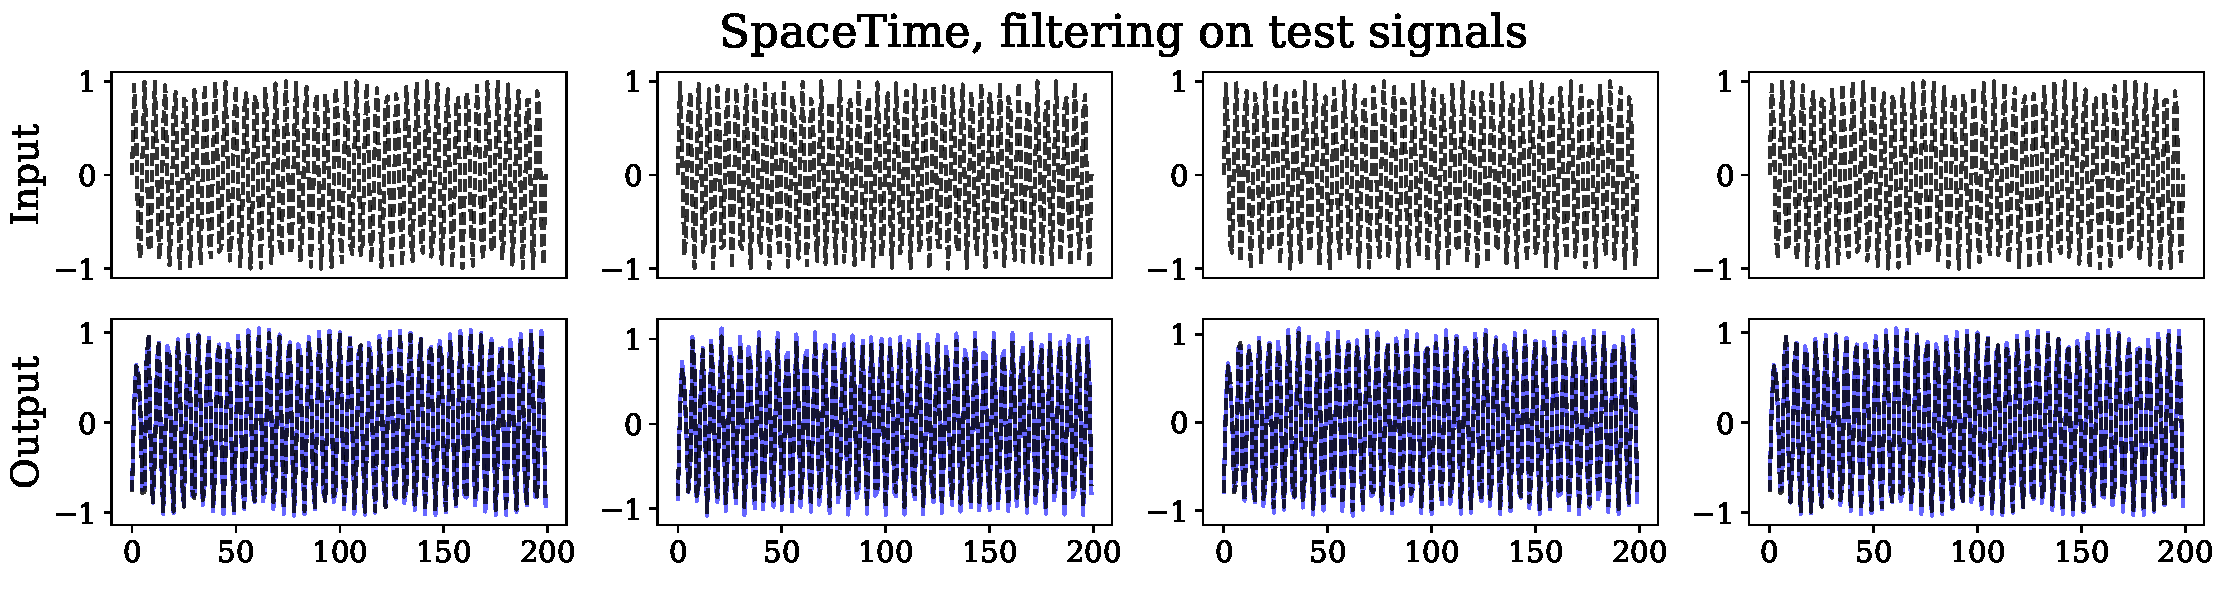
\includegraphics[width=0.99\columnwidth]{_ICLR2023_paper/figures/dsp_SpaceTime.pdf}
%     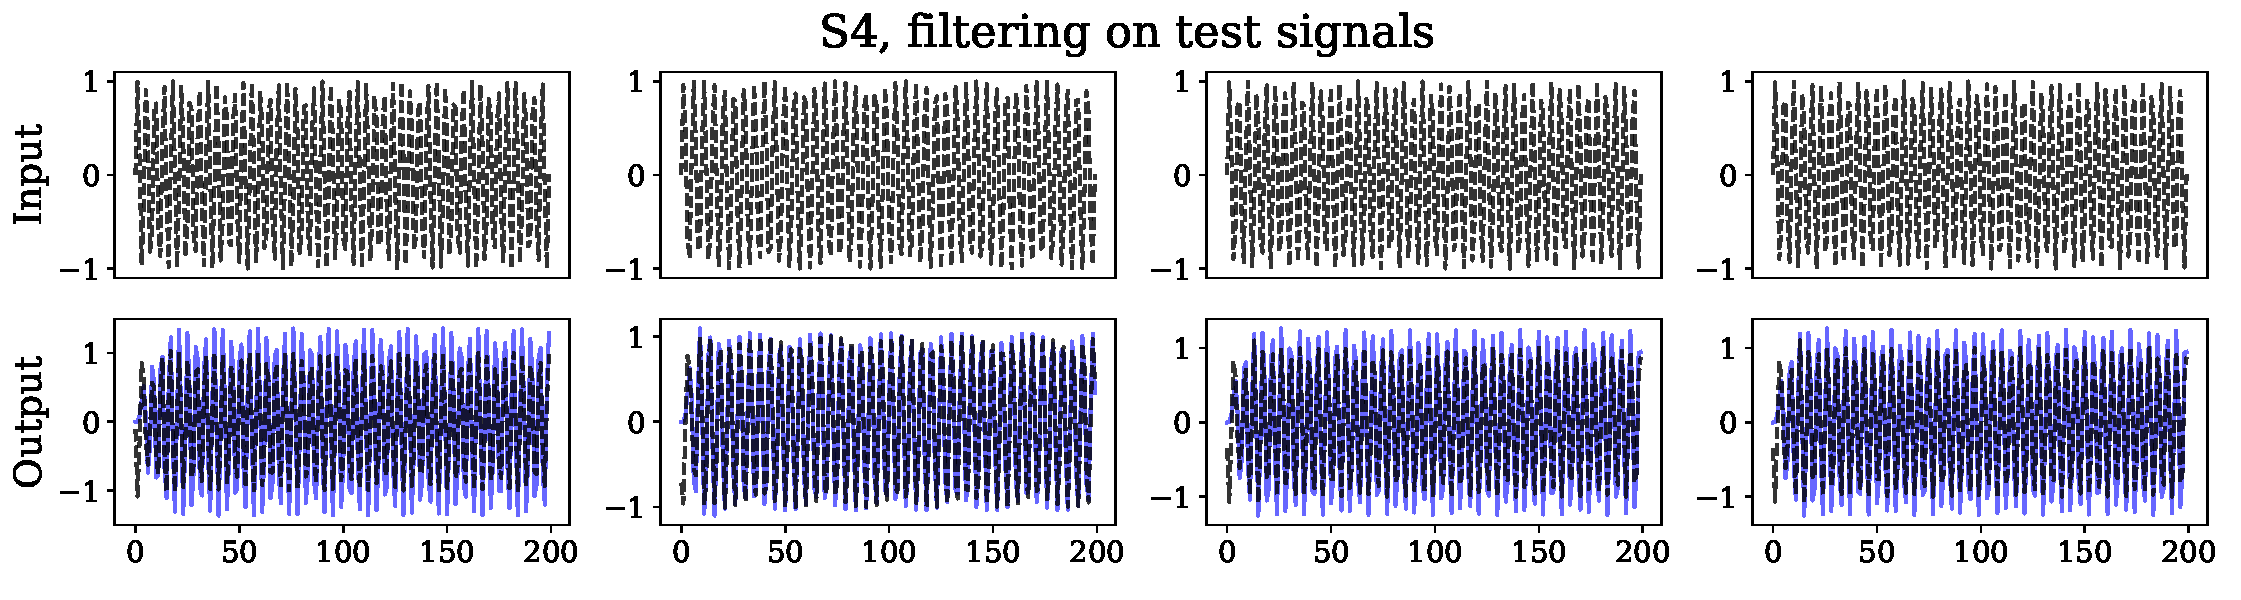
\includegraphics[width=0.99\columnwidth]{_ICLR2023_paper/figures/dsp_S4.pdf}
%     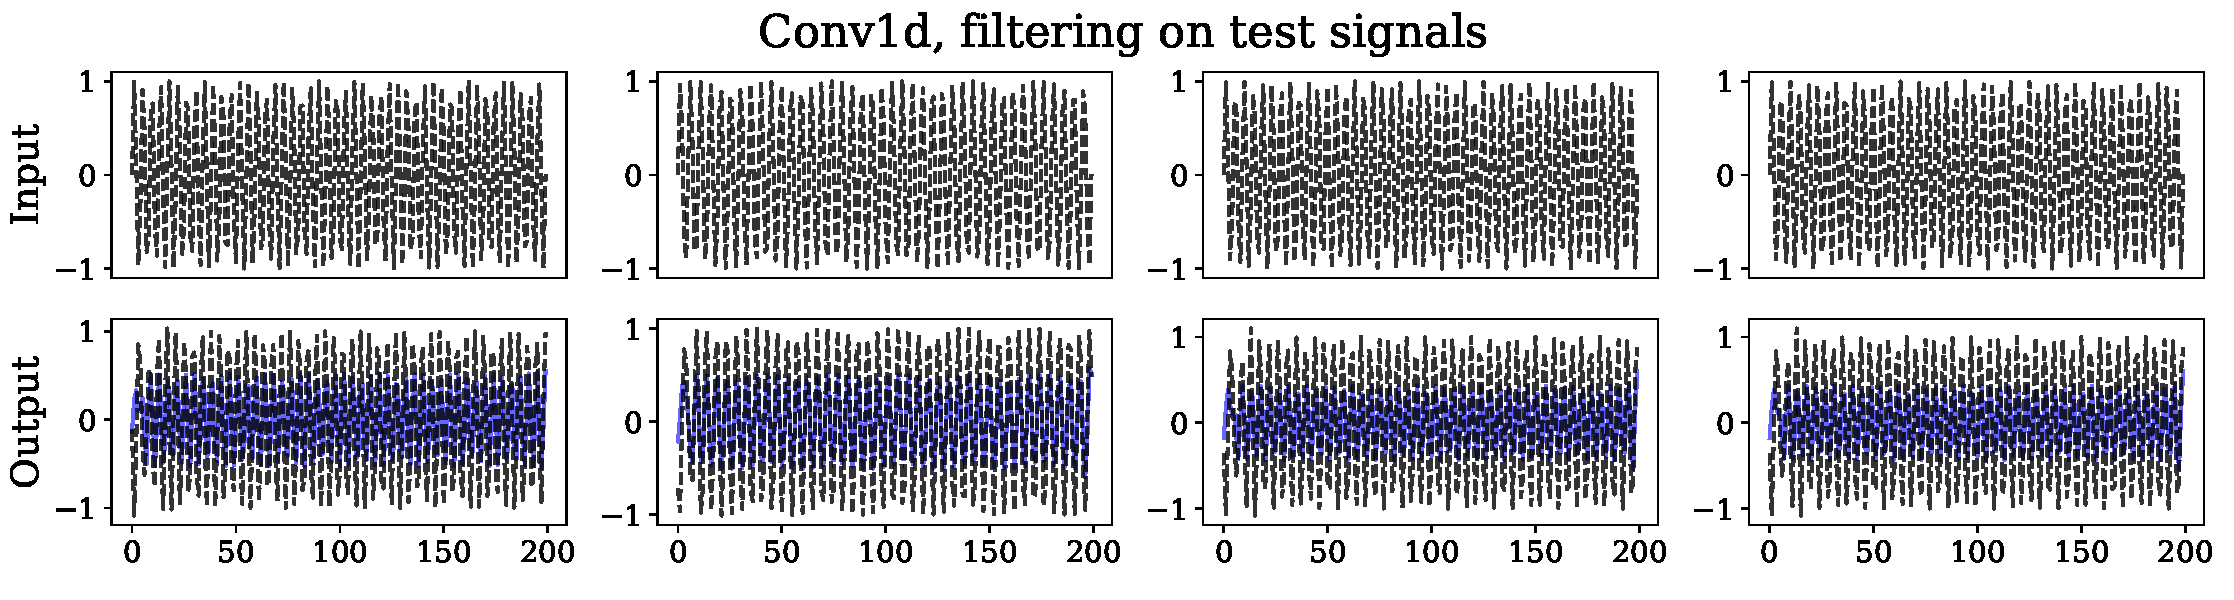
\includegraphics[width=0.99\columnwidth]{_ICLR2023_paper/figures/dsp_Conv1d.pdf}
%     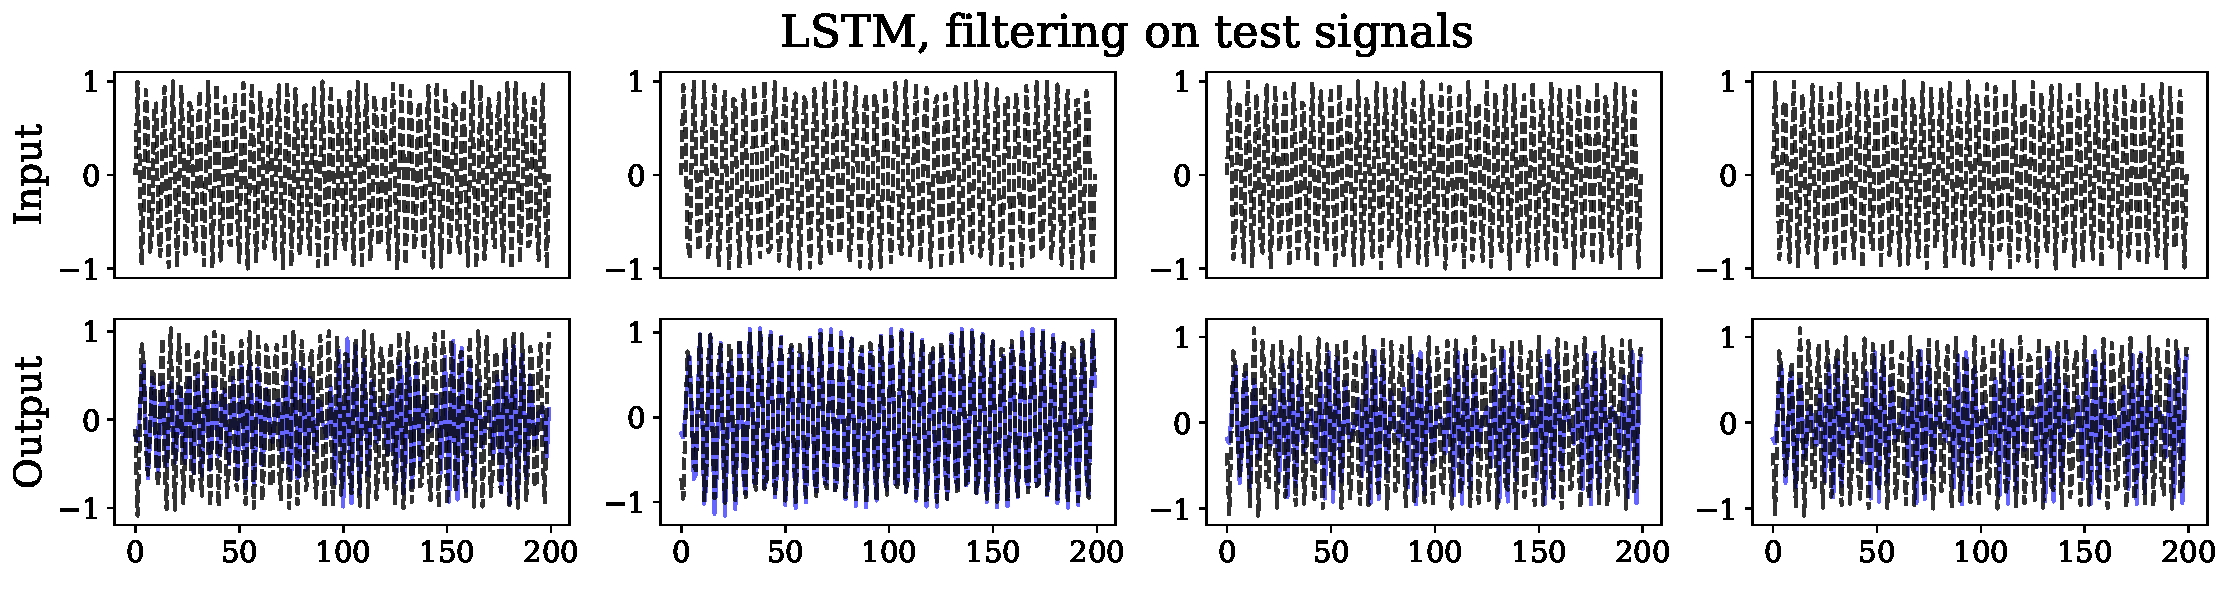
\includegraphics[width=0.99\columnwidth]{_ICLR2023_paper/figures/dsp_LSTM.pdf}
%     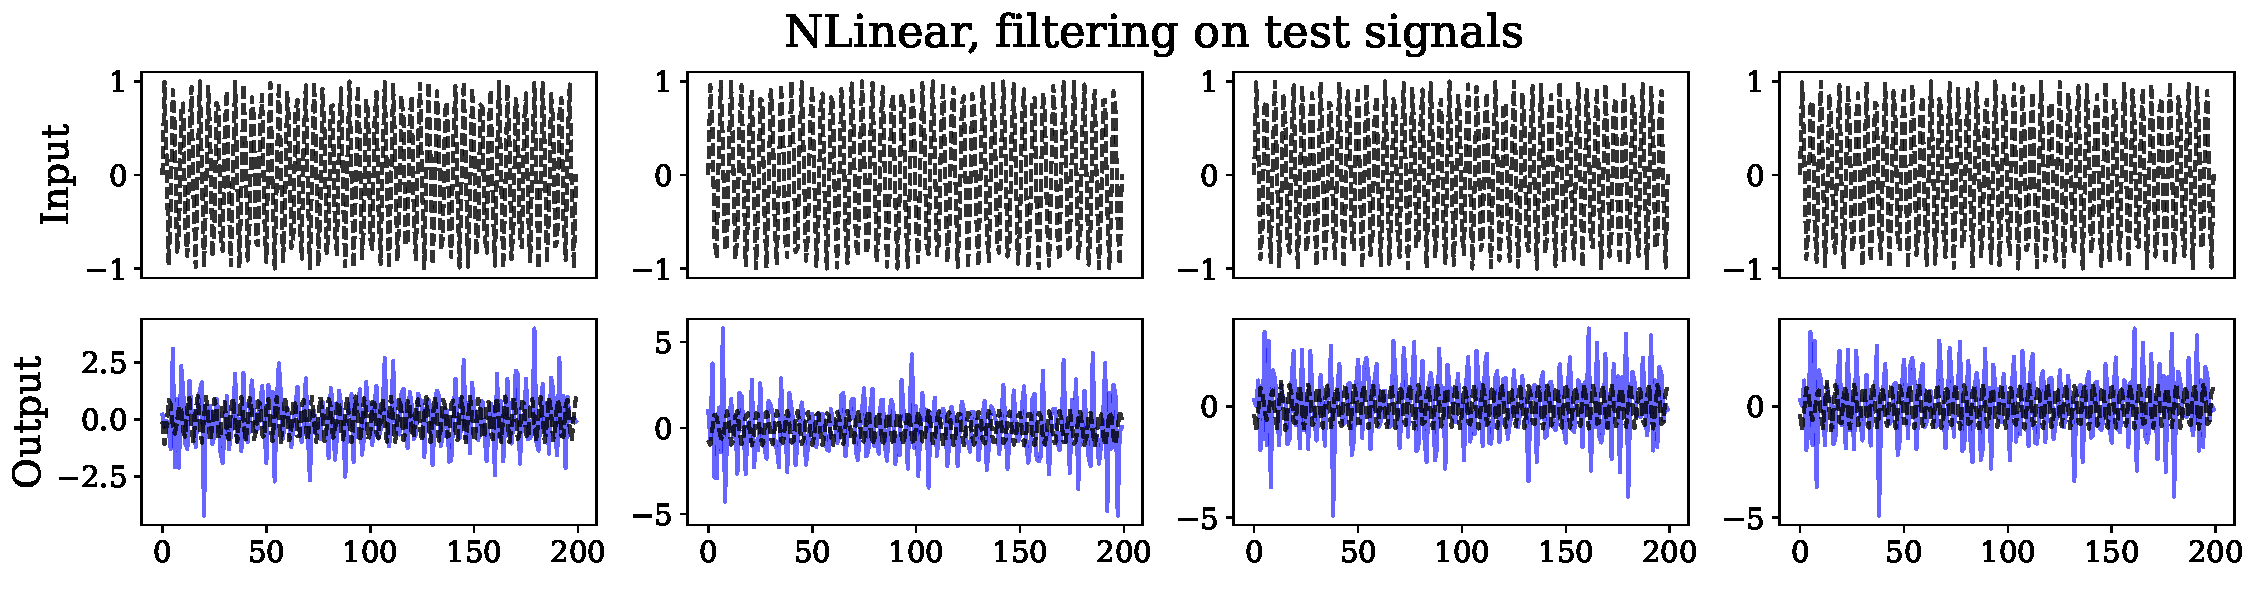
\includegraphics[width=0.99\columnwidth]{_ICLR2023_paper/figures/dsp_NLinear.pdf}
%     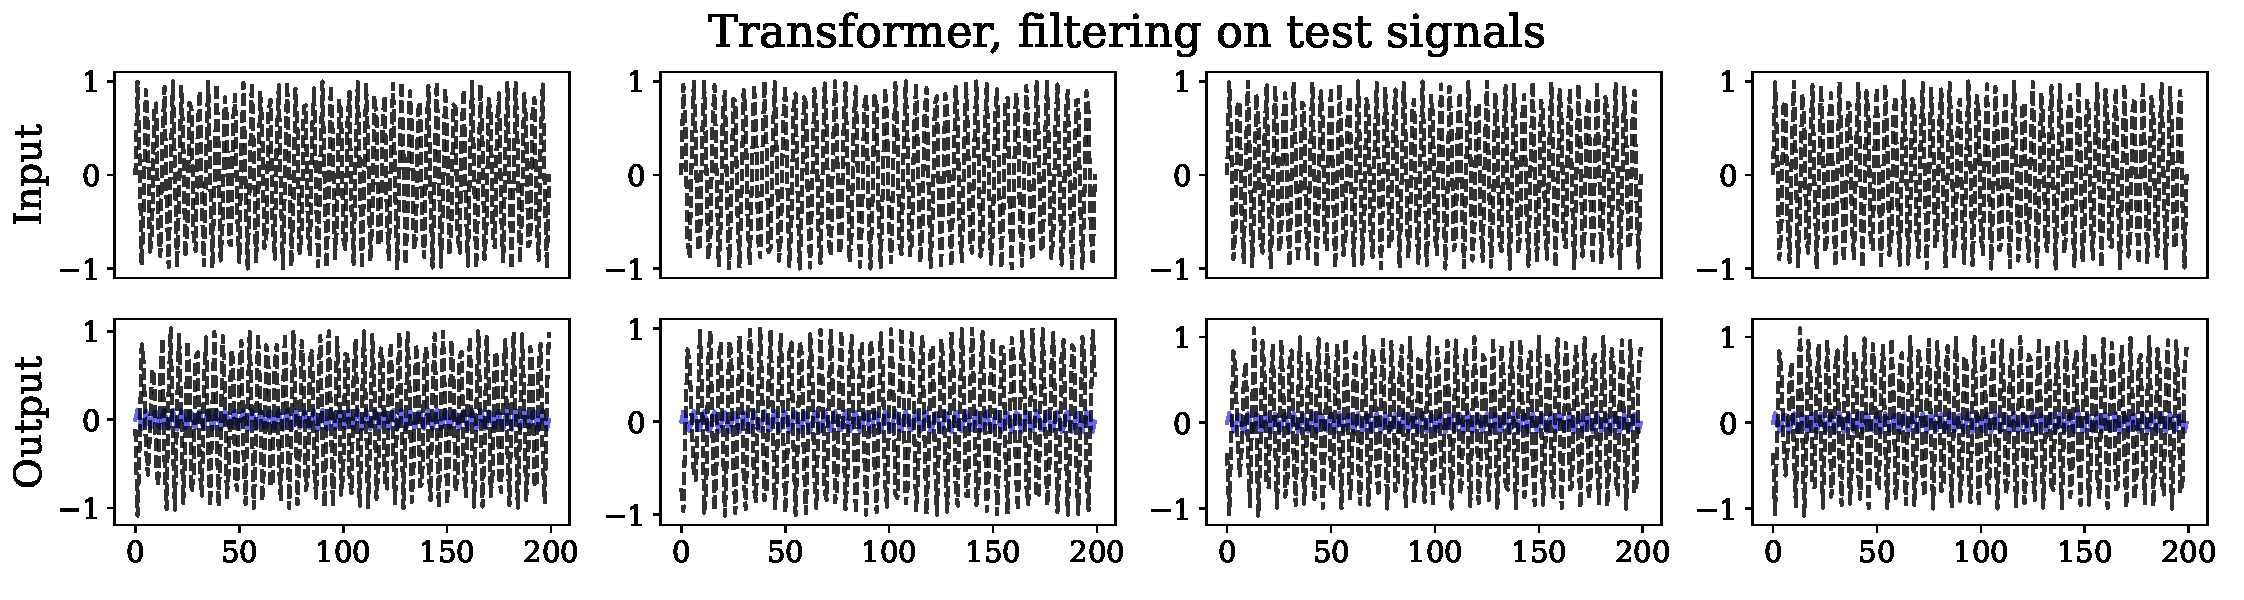
\includegraphics[width=0.99\columnwidth]{_ICLR2023_paper/figures/dsp_Transformer.pdf}
%     \vspace{-2mm}
%     \caption{Testing the capability of different sequence--to--sequence models to approximate the input--output map of digital filters. In blue, we show the output signal filtered by each model. The ground--truth digital filter is a Butterworth of order $10$.}
%     \label{fig:dsp_synthetic}
% \end{figure}
% %


% \begin{sidewaystable}[t]
%     \small
%     \centering
%     \begin{tabular}{c|c|cccccc|ccccc}
%     \toprule
%     %
%     Dataset  & \ourmethod & SES & Theta & TBATS & ETS & (DHR-)ARIMA & PR & CatBoost & DeepAR & N-BEATS & WaveNet & Transformer \\
%     %
%     \midrule
%     M1 Yearly & \underline{135508.3} & 193829.5 & 171458.1 & \textbf{116850.9} & 167739.0 & 175343.8 & 152038.7 & 237644.5 & 173075.1 & 192489.8 & 312821.8 & 182850.6 \\
    
%     M1 Quarterly & \underline{2200.3} & 2545.7&	2282.7	&2673.9&	2408.5&	2538.5&	1909.3&	2161.0& 2313.3&	2267.3&	2271.7&	2231.5  \\    
    
%     M1 Monthly & 2601.1 & 2725.8 & 2564.9 & 2594.5 & 2264.0 & 2450.6 & 2478.8 & 2461.7 & 2202.2 & \textbf{2183.4} & 2578.9 & 3129.8  \\

%     M3 Yearly & 1412.4 & 1172.9&	1106.1&	1386.3	&1189.2	&1662.2	&1181.8&	1341.7&		1157.9&	1117.4&	1147.6&	1084.8 \\
    
%     M3 Quarterly & 676.1 & 670.6&	567.7&	653.6&	598.7&	650.8&	605.5&	698.0&	606.6&	582.8&	606.8&	819.2\\ 
    
%     M3 Monthly & 897.12 & 893.9	&754.0&	765.2	&755.3&	790.8&	830.0&	874.2&	873.7&	796.9&	845.3&	948.4 \\
    
%     M3 Other & 265.56 & 309.7	&242.1&	217.0&	224.1	&220.8	&262.3&	349.9&	277.7&	248.5&	277.0	&271.0 \\
    
%     M4 Quarterly & 718.2 & 732.8&	673.2&	672.7&	674.3&	710.0&	711.9&	714.2&	700.3&	684.7&	697.0&	739.1 \\
    
%     M4 Monthly & 1092.2 & 755.5	&683.7&	743.4&	705.7&	702.1&	720.5&	734.8&	740.3&	705.2&	787.9&	902.4\\ 
    
%     M4 Weekly & \textbf{348.3}& 412.6	&405.2&	356.7&	408.5	&386.3&	350.3&	420.8&	422.2&	330.8&	437.3&	456.9\\ 
    
%     M4 Daily &\textbf{183.2}& 209.8&	210.4&	\underline{208.4}&	230.0	&212.6&	213.0&	263.1	&343.5&	221.7&	220.5&	233.6\\ 
    
%     M4 Hourly & \textbf{255.2} & 1476.8	&1483.7	&469.9&	3830.4&	1563.1&	\underline{313.0} &	344.6&	1095.1&	501.2&	468.1&	391.2\\
    
%     Tourism Yearly & \textbf{74799.2}& 106665.2&	99914.2&	105799.4&	104700.5&	106082.6&	89645.6	&87489.0&	78470.7&	78241.7	&77581.3&	80089.3\\
    
%     Tourism Quarterly & 11608.32& 15000.0&	9254.6&	12001.5	&10812.3	&12564.8	&11746.9	&12788.0	&11762.0&	11306.0	&11546.6	&11724.1 \\
    
%     Tourism Monthly & 3181.2& 7039.4&	2702.0	&3661.5	&2543.0	&3132.4&	2739.4&	3102.8&	2359.9&	2596.2&	2694.2&	2660.1\\
    
%     Pedestrian & 69.6& 228.1&	228.2	&261.3&	278.3&	820.3&	61.8&	60.8&	65.8&	99.3&	68.0&	70.2\\
    
%     Weather & \textbf{2.7}& 2.9	&3.3&	2.9&	3.0&	3.1	&9.1&	3.1&	\textbf{2.7}	&3.1&	3.0	&2.8\\
    
%     NN5 Weekly & \textbf{16.9}& 18.8&	18.7&	18.5&	18.8&	18.6&	18.6&	18.7&	18.5&	17.4&	24.2&	24.0 \\
    
%     Solar $10$ min &7.4& 7.2&	7.2	&10.7&	7.2	&5.6&	7.2	&8.7&	7.2	&6.6&	8.0&	7.2\\
    
%     Solar Weekly &1423.7& 1331.3&	1341.6&	1049.0&	1264.4&	967.9&	1168.2&	1754.2&	873.6&	1307.8&	2569.3&	693.8\\
    
%     Electricity Hourly & \textbf{475.1} & 1026.3&	1026.4&	743.4&	1524.9&	1082.4&	689.9&	582.7&	\underline{478.0} &	510.9&	489.9&	514.7\\
    
%     Electricity Weekly &37802.2& 77067.9&	76935.6&	28039.7	&70369.0&	32594.8&	47802.1&	37289.7	&53100.3&	35576.8	&63916.9&	78894.7\\
    
%     Fred-MD &3743.6& 3103.0&	3898.7&	2295.7&	2341.7	&3312.5&	9736.9&	2679.4&	4638.7&	2813.0&	2779.5&	5098.9\\
    
%     Traffic Hourly &0.03& 0.04&	0.04	&0.05&	0.04	&0.04&	0.03	&0.03&	0.02&	0.02	&0.03&	0.02\\
    
%     Traffic Weekly &\textbf{1.3}& 1.5&	1.5	&1.5&	1.5	&1.5&	1.5&	1.5	&1.5&	1.4	&1.6&	1.9\\
    
%     Hospital &40.1& 26.6&	22.6&	21.3&	22.0	&23.7&	23.5&	23.5&	22.0&	24.2&	23.4&	40.5\\
    
%     Covid &490.1& 403.4&	370.1&	113.0&	102.1&	100.5&	394.1&	607.9&	230.5&	186.5&	1135.4&	480.0\\
    
%     Saugeen & \textbf{24.0} & 39.8	&39.8	&42.6&	50.4&	43.2&	47.7&	\underline{39.3} &	45.3&	48.9&	43.0&	49.1\\
    
%     US Births &630.2& 1369.5&	735.5&	606.5&	607.2&	705.5&	732.1&	618.4&	684.0&	627.7&	768.8&	686.5\\
    
%     Sunspot &3.1& 5.0	&5.0&	3.0	&5.0&	3.0	&4.0&	2.4	&1.1&	14.5&	0.7	&0.5\\
    
%     Car Parts & 0.64 & 0.71&	0.65	&0.71&	0.71&	0.71&	\underline{0.58}&	0.71&	\textbf{0.50}&	1.0&	\underline{0.58}&	0.5\\
    
%     Vehicle Trips &30.4& 36.5&	37.4&	25.7&	37.6&	35.0&	31.7&	27.3&	26.5&	33.6&	29.0&	33.0\\
%     \bottomrule
%     %
%     \end{tabular}
%     \caption{Monash forecasting. We report test RMSE of \ourmethod for each dataset (best result selected via validation RMSE, average of $3$ runs).}
%     \label{tab:monash}
% \end{sidewaystable}


% \begin{table}[t]
%     \small
%     \centering
%     \begin{tabular}{c|cccc}
%     \toprule
%     %
%     Dataset  & Ours & S4S & S4D & S4DPLR  \\
%     %
%     \midrule
%     M1 Yearly & {\color{red!50}$154770.78$} & {\color{red!50}$177978.63$} & $161463.53$ &  \\
%     M1 Quarterly \\
%     M1 Monthly \\
%     M3 Yearly \\
%     M3 Quarterly \\ 
%     M3 Other \\ 
%     M4 Monthly \\ 
%     M4 Weekly \\ 
%     M4 Daily \\ 
%     Tourism Yearly \\
%     Tourism Monthly \\
%     Dominick \\
%     Pedestrian \\
%     Weather
%     NN5 \\
%     Solar $10$ min & $6.72$ &\\
%     Solar Weekly \\
%     Electricity Hourly \\
%     Electricity Weekly \\
%     Fred-MD \\
%     Traffic Hourly \\
%     Traffic Weekly \\
%     Hospital \\
%     Covid \\
%     Saugeen \\
%     US Births \\
%     \bottomrule
%     %
%     \end{tabular}
%     \caption{Monash forecasting. We report average test RMSE of \ourmethod for each dataset ($5$ runs each).}
%     \label{tab:my_label}
% \end{table}


% \begin{sidewaystable}[t]
%     \small
%     \centering
%     \begin{tabular}{c|c|cccccc|ccccc}
%     \toprule
%     %
%     Dataset  & Ours & SES & Theta & TBATS & ETS & (DHR-)ARIMA & PR & CatBoost & FFNN & DeepAR & N-BEATS & WaveNet & Transformer \\
%     %
%     \midrule
%     M1 Yearly & $2$ & $11$ & $6$ & $1$ & $5$ & $8$ & $3$ & $12$ & $4$ & $7$ & $10$ & $13$ & $9$ \\
%     M1 Quarterly \\
%     M1 Monthly \\
%     M3 Yearly \\
%     M3 Quarterly \\ 
%     M3 Other \\ 
%     M4 Monthly \\ 
%     M4 Weekly \\ 
%     M4 Daily \\ 
%     Tourism Yearly \\
%     Tourism Monthly \\
%     Dominick \\
%     Pedestrian \\
%     Weather
%     NN5 \\
%     Solar $10$ min & $6.72$ &\\
%     Solar Weekly \\
%     Electricity Hourly \\
%     Electricity Weekly \\
%     Fred-MD \\
%     Traffic Hourly \\
%     Traffic Weekly \\
%     Hospital \\
%     Covid \\
%     Saugeen \\
%     US Births \\
%     \bottomrule
%     %
%     \end{tabular}
%     \caption{Monash foreacasting. Model rankings (based on test RMSE).}
%     \label{tab:my_label}
% \end{sidewaystable}